\documentclass[CJK]{beamer}
\usepackage{CJKutf8}
\usepackage{beamerthemesplit}
\usetheme{Malmoe}
\useoutertheme[footline=authortitle]{miniframes}
\usepackage{amsmath}
\usepackage{amssymb}
\usepackage{graphicx}
\usepackage{color}
\usepackage{slashed}
\usepackage{simplewick}
\graphicspath{{../figures/}}
\def\be{\begin{equation}}
\def\ee{\nonumber\end{equation}}
\def\bea{\begin{eqnarray}}
\def\eea{\nonumber\end{eqnarray}}
\def\ii{{\dot{\imath}}}
\def\bch{\begin{CJK}{UTF8}{gbsn}}
\def\ech{\end{CJK}}
\def\bex{\begin{minipage}{0.3\textwidth}
\includegraphics[width=1in]{jugelizi.png}\end{minipage}\begin{minipage}{0.6\textwidth}}
\def\eex{\end{minipage}}
\def\chtitle#1{\frametitle{\bch#1\ech}}
\def\skipline{{\vskip0.1in}}
\def\skiplines{{\vskip0.2in}}
\def\lagr{{\mathcal{L}}}
\def\hamil{{\mathcal{H}}}
\def\vecv{{\mathbf{v}}}
\def\vecx{{\mathbf{x}}}
\def\veck{{\mathbf{k}}}
\def\vecp{{\mathbf{p}}}
\def\vecn{{\mathbf{n}}}
\def\vecA{{\mathbf{A}}}
\def\vecP{{\mathbf{P}}}
\def\vecsigma{{\mathbf{\sigma}}}
\def\hatJn{{\hat{J_\vecn}}}
\def\hatJx{{\hat{J_x}}}
\def\hatJy{{\hat{J_y}}}
\def\hatJz{{\hat{J_z}}}
\def\hatj#1{\hat{J_{#1}}}
\def\hatphi{{\hat{\phi}}}
\def\hatq{{\hat{q}}}
\def\hatpi{{\hat{\pi}}}
\def\vel{\upsilon}
\def\Dint{{\mathcal{D}}}
\def\adag{{\hat{a}^\dagger}}
\def\bdag{{\hat{b}^\dagger}}
\def\cdag{{\hat{c}^\dagger}}
\def\ddag{{\hat{d}^\dagger}}
\def\hata{{\hat{a}}}
\def\hatb{{\hat{b}}}
\def\hatc{{\hat{c}}}
\def\hatd{{\hat{d}}}
\def\hatN{{\hat{N}}}
\def\hatH{{\hat{H}}}
\def\hatp{{\hat{p}}}
\def\Fup{{F^{\mu\nu}}}
\def\Fdown{{F_{\mu\nu}}}
\def\newl{\nonumber \\}
\def\SIkm{\mathrm{km}}
\def\SIyr{\mathrm{yr}}
\def\SIGyr{\mathrm{Gyr}}
\def\SIeV{\mathrm{eV}}
\def\SIGeV{\mathrm{GeV}}
\def\SIm{\mathrm{m}}
\def\SIcm{\mathrm{cm}}
\def\SIJ{\mathrm{J}}
\def\SIs{\mathrm{s}}
\def\SIkg{\mathrm{kg}}
\def\SIg{\mathrm{g}}
\def\vece{\mathrm{e}}
\def\bmat#1{\left(\begin{array}{#1}}
\def\emat{\end{array}\right)}
\def\bcase#1{\left\{\begin{array}{#1}}
\def\ecase{\end{array}\right.}
\def\calM{{\mathcal{M}}}
\def\calT{{\mathcal{T}}}
\def\calR{{\mathcal{R}}}
\def\barpsi{\bar{\psi}}
\def\baru{\bar{u}}
\def\barv{\bar{\upsilon}}
\def\bmini#1{\begin{minipage}{#1\textwidth}}
\def\emini{\end{minipage}}
\def\qeq{\stackrel{?}{=}}
\def\torder#1{\mathcal{T}\left(#1\right)}
\def\rorder#1{\mathcal{R}\left(#1\right)}


\title{Quantum Field Theory I \\ Lesson 13 - The Second Feynman diagram}
\author{}
\date{}


\begin{document}

\begin{frame}
 
\begin{center}
\begin{Large}
\bch
量子场论 I 

{\vskip 0.3in}

第十三课 第二个Feynman图

\ech
\end{Large}
\end{center}

\vskip 0.2in

\bch
课件下载
\ech
https://github.com/zqhuang/SYSU\_QFTI

\end{frame}


\begin{frame} 
\chtitle{三次相互作用} 
\bch
考虑拉氏密度为
$$\lagr = \frac{1}{2}\partial^\mu\phi\partial_\mu\phi - \frac{1}{2}m^2\phi^2 - \frac{g}{3!}\phi^3- \frac{\lambda}{4!}\phi^4$$
的实标量场。其中$\lambda>0$和$g$都是耦合常数。我们仅考虑它很小($\lambda \ll 1$, $g\ll m$)的情况。

我们取如下的相互作用表象:
$$ H_0 = H_{\rm free},\ H_I = \frac{\lambda}{4!} \int d^3\vecx\, \phi^4$$
其中$H_{\rm free} = \int d^3\vecx\, \frac{1}{2}(\dot\phi^2 + |\nabla \phi|^2 + m^2\phi^2)$是我们以前学过的自由场的Hamilton量。

\ech
\end{frame}

\begin{frame} 
\chtitle{热身问题} 
\bch
我们的热身问题是:

求两个动量为$\vecp_1$, $\vecp_2$的粒子发生散射,变为两个动量为$\vecp_3$, $\vecp_4$的粒子的概率幅。
$$\calM T/V= \langle \vecp_3, \vecp_4|  e^{-\ii\int_{-\infty}^\infty \hat{H}_I dt}|\vecp_1,\vecp_2\rangle$$
空间总体积$V\rightarrow \infty$和总时间长度$T\rightarrow \infty$。我们在定义概率振幅时引入了$T/V$的因子来描述空间越大两个自由粒子越难碰到发生散射,以及时间越长越越容易发生散射。在最后的表达式中两边会约去$T/V$。

为了讨论简单起见,我们假设这四个动量$\vecp_1$, $\vecp_2$, $\vecp_3$, $\vecp_4$互不相同。
\ech
\end{frame}

\begin{frame} 
\chtitle{一阶微扰展开} 
\bch

我们做一阶微扰展开:
$$e^{-\ii\int_{-\infty}^\infty \hat{H}_I dt}\approx 1 -\ii\int_{-\infty}^\infty \hat{H}_I dt = 1-\ii\int d^4x\, \frac{\lambda}{4!}\hat\phi^4 $$

若末态与初态不同则第一项$1$没有贡献。我们来计算最低阶的非零贡献:
$$\calM T/V \approx -\ii \langle \vecp_3, \vecp_4| \int d^4x\, \frac{\lambda}{4!}\hat\phi^4 |\vecp_1,\vecp_2\rangle$$

\ech
\end{frame}

\begin{frame} 
\chtitle{写成产生湮灭算符} 
\bch

{\small
由于该相互作用表象下$\hatphi$仍按$d\hat\phi/dt = - \ii [\hatphi,  \hatH_{\rm free}]$演化,$\hatphi$的解就和自由场相同
$$\hatphi = \frac{1}{(2\pi)^{3/2}}\int \sqrt{\frac{d^3\veck}{2\omega}} \left(\hata_{\veck}e^{-ikx}+\adag_{\veck}e^{ikx}\right)$$
代入要求解的概率幅后得到
\be
\calM T/V \approx \frac{-\ii\lambda}{4!(2\pi)^6} \int d^4x \langle \vecp_3, \vecp_4|\left[\int \sqrt{\frac{d^3\veck}{2\omega}} \left(\hata_{\veck}e^{-ikx}+\adag_{\veck}e^{ikx}\right)\right]^4 |\vecp_1,\vecp_2\rangle
\ee
显然,要使得矩阵元非零,在四个括号里必须分别取出动量为$\vecp_1$, $\vecp_2$的湮灭算符以及动量为$\vecp_3$, $\vecp_4$的产生算符。这样一共有$4!$种取法,刚好和外面分母里的$4!$抵消了,于是得到:
\be
\calM T/V \approx \frac{-\ii\lambda}{(2\pi)^6} \int d^4x\, \frac{(d^3\veck)^2}{4\sqrt{\omega_1\omega_2\omega_3\omega_4}} e^{-i(p_1+p_2-p_3-p_4)x} 
\ee
}
\ech
\end{frame}

\begin{frame} 
\chtitle{化简} 
\bch
{\small
利用四维空间的积分公式:
$$\frac{1}{(2\pi)^4}\int d^4 x\, e^{-i(p_1+p_2-p_3-p_4)x} = \delta(p_1+p_2-p_3-p_4)$$
我们最终得到:
\be
\calM T/V \approx \frac{-\ii\lambda}{(2\pi)^2} \frac{(d^3\veck)^2}{4\sqrt{\omega_1\omega_2\omega_3\omega_4}} \delta(p_1+p_2-p_3-p_4)
\ee
注意到$d^3\veck = (2\pi)^3/V$(例如考虑一个边长为$L$的立方盒子),以及$d^4k = (2\pi/T)d^3\veck$,我们可以把上式写成
\be
\calM \approx -\ii\lambda \frac{1}{4\sqrt{\omega_1\omega_2\omega_3\omega_4}} \delta(p_1+p_2-p_3-p_4)d^4k
\ee
}
\ech
\end{frame}

\begin{frame} 
\chtitle{对结果的物理讨论} 
\bch
{\small
结果中的$\delta(p_1+p_2-p_3-p_4)d^4k$在$p_1+p_2-p_3-p_4=0$时为1,否则为零。这是散射问题能量动量守恒的自然结果。一般定义散射振幅时会把这个能量动量守恒因子排除在外,按这样的定义方法,最后结果就是:
\be
\calM \approx -\ii\lambda \frac{1}{4\sqrt{\omega_1\omega_2\omega_3\omega_4}} 
\ee
}
\ech
\end{frame}

\begin{frame} 
\chtitle{这个问题对应的Feynman图和Feynman规则} 
\bch
\begin{minipage}{0.45\textwidth}
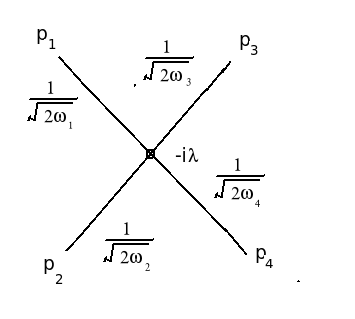
\includegraphics[width=2in]{Feynman_lf4_tree.png}
\end{minipage}
\begin{minipage}{0.45\textwidth}
实标量场$\frac{\lambda}{4!}\phi^4$相互作用项的Feynman规则:
\begin{itemize}
\item{四线交叉顶角给出因子$-\ii\lambda$}
\item{每条外线给出因子$1/\sqrt{2\omega}$}
\end{itemize}
\end{minipage}

\ech
\end{frame}

\begin{frame}
\chtitle{选择题时间} 
\bch
我们算完了人生中第一个Feynman图,你的感想是:
\begin{itemize}
\item[A]{无敌是多么寂寞}
\item[B]{老师你故意找个最好算的图逗我们的吧!}
\item[C]{刚才发生了什么……}
\end{itemize}
\ech
\end{frame}

\begin{frame}
\chtitle{答案是B} 
\bch

下节课我们要动真格的了。
\ech
\end{frame}

\end{document}


